% Document Purpose
\documentclass{report}

% Packages
\usepackage{amsmath}
\usepackage{amssymb}
\usepackage{enumerate}
%%%%%%%%%%%%%%%%%%%%%%%%%%%%%

\title{McQuarrie Stat Mech Notes}
\author{Brandon Butler}
\date{2019--04--02}

% User defined commands
\renewcommand{\d}{\text{d}}
\newcommand{\note}{\textit{Note:} }
\newcommand{\H}{\mathcal{H}}
\newcommand{\Q}{\mathcal{Q}}
\begin{document}

\chapter{Canonical Ensemble}
% Chapter 2 Notes

\subsection{Assumptions}

\begin{itemize}

	\item No uncertainty in energy states.

	\item Each system is a pure system.

	\item An isolated system is equally likely to be in any available state.

	\item The average of a property over all available microstates is the
		macroscopic value.

\end{itemize}

\section{MicroCanonical}\label{sec:ch2MicroCanonical}

For a system with constant number, volume, and energy, the number of microstates
is \[ \Omega = \Omega(N, V, E).\]

Now take an ensemble or collection of systems like this with the number of
systems in the ensemble being $A$. Then, \[ E_{tot} = A E
\]\[N_{tot} = A N \] \[ V_{tot} = A V.\]  Since we have no reason to favor one
system over the other, we assume each state with the same $N, V, E$ is equally
probable. This is known as the principle of equal \textit{a priori}
probabilities. 

\section{Canonical}\label{sec:Canonical}

\subsection{Deriving the Partition Function}

Now lets take a ensemble of systems with the same temperature, volume, and
number. The ensemble is put into a heat bath until it is fully equilibrated,
and then moved into perfect thermal insulation. The entire ensemble then becomes
a system in the microcanonical ensemble.

We know that the system must obey,
\[ A = \sum_j{a_j} \]\[ E_{tot} = \sum_j{a_j E_j},\]
where  $a_j$ is the occupancy number of state j. We generally do not know the
occupancy number of states or number of states, however.

We do know (assumption) that for the microcanonical ensemble each state is
equally likely. This means that each state for the entire canonical ensemble is
equally likely since the entire canonical ensemble is a system in the
microcanonical ensemble; that is all combinations of occupancy numbers is
equally likely.

The number of states with distribution $\vec{a}$ of occupancy numbers is given
by
\[ W(\vec{a}) = \frac{A!}{ \prod_{j}{a_j!}}.\]
This a multinomial coefficient meaning that at large $A$ it is very sharply
peaked; in fact, arbitrarily so at large enough $A$. The probability of being in
state j is,
\[ P_j =  \frac{\sum_a{W(\vec{a})a_j(\vec{a})}}{A \sum_a{W(\vec{a})}}
= \frac{\bar{a_j}}{A}.\]
At infinite number of systems in an ensemble, all contributions besides the most
common become completely negligible, thus
\[ P_j = \frac{\bar{a_j}}{A} = \frac{a_j^{*}}{A}.\] 

We now have a maximization problem (maximizing the weight function $W$) with the
following constraints.
\[ A = \sum_{j}{a_j} \]
\[ E_{tot} = \sum_{j}{a_j E_j}.\]

Since $\ln$ is a monotonic function and, thus, will preserve maxima and minima of
inputted functions, $\ln(W(\vec{a}))$ can be maximized instead of $W(\vec{a})$.
For further calculations it behooves us to recognize that
\[ \ln(W) = \ln(A!) - \sum_j{\ln(a_j!)}.\]
Note the first term is constant and the second is approximately
\[-\sum_j{a_j \ln(a_j)} + \sum_{j}{a_j} = -\sum_j{a_j \ln(a_j)} + A.\]
Using this we take the partial differential,
\[ \frac{\partial ( \ln W(\vec{a}) - \alpha \sum_{j}{a_j} - \beta \sum_j{a_j
E_j})}{\partial a_{k}} = 0, \]
for each $k$ and find,
\[ \ln(a^*_k)+ \alpha + 1 + \beta E_k = 0 \]
or
\[ a_k^* = e^{-\alpha^{'}}e^{-\beta E_{k}}, \text{where} \alpha^{'} = \alpha +
1. \]
Summing over all $(a_j^*)$ gives,
\[ A = e^{ -\alpha^{'}}\sum_{j}{e^{ - \beta E_j}}. \]
Finally,
\[ P_j = \frac{e^{-\alpha^{'}}e^{-\beta E_{k}}}{e^{ -\alpha^{'}}\sum_j{e^{
-\beta E_{j}}}} = \frac{e^{-\beta E_k}}{\sum_j{e^{ -\beta E_j}}}.\]

We call the denominator $Q$ and label it the partition function. We now show
the ensemble energy and some of its derivatives.

\subsection{Finding $\beta$}

\[\bar{E} = \frac{\sum_{j}{E_j e^{-\beta E_{j}}}}{Q}.\]
\[ p_j = - \left(\frac{\partial E}{\partial V}\right)_N.\]
\[ \bar{p} = - \frac{\sum_j{\left( \frac{\partial E}{\partial V} \right)_{N}
e^{-\beta E_j}}}{Q}.\]

We can then find,
\[ \left( \frac{ \partial \bar{E} }{ \partial V}\right)_{N, \beta} = -\bar{p}
+ \beta \overline{Ep} - \beta \bar{E} \bar{p} \] and
\[ \left( \frac{ \partial \bar{p} }{ \partial \beta }\right)_{N, V} =
\bar{E}\bar{p} - \overline{Ep}.\]

Comparing the thermodynamic and ensemble averages we see,
\[\left( \frac{ \partial \bar{E} }{ \partial V}\right)_{N, \beta} +
\beta \left( \frac{ \partial \bar{p} }{ \partial \beta }\right)_{N, V} =
- \bar{p},\]

\[\left( \frac{ \partial E }{ \partial V}\right)_{N, T} -
T \left( \frac{ \partial p }{ \partial T }\right)_{N, V} = - p.\]

One can see from this that $ \beta = \frac{k}{T} $. k will be the same for any
system as can be seen from a thought experiment where the ensemble consists of
two system composites with the same $N, V, T$. They individual systems will be
in equilibrium and from prior calculations the partition function and
probability functions are completely separable. This requires they have the same
constant k.

\subsection{Entropy}

Let \[f = \ln Q.\] Then, \[ df = \left( \frac{ \partial f }{ \partial \beta }
\right)_{E_{j}} d \beta + \sum_{k}{\left( \frac{ \partial f }{ \partial E_{k}}
\right)_{\beta, E_{j \neq k}} d E_{k}}.\] 
This derivative is equivalent of slightly changing the volumes of all systems
which changes the energy levels (which is nothing but PV work) and slightly
change the temperature before isolated the ensemble again.

This becomes with some manipulation,
\[ df = -\bar{E} d \beta - \beta \sum_{k}{P_{k} dE_{k}} \]
\[ d(f + \beta \bar{E}) = \beta \left( d \bar{E} - \sum_{k}{P_{k} dE_{k}}
\right).\]

The first term is the change in average system energy, while the second is the
average change of energies in corresponding energy levels. The first is a total
energy change while the second is average reversible work. Thus, the quantity is
the average reversible heat that of system. This requires that
$\beta$ is an integrating factor of $f$.  \[ d(f + \beta \bar{E}) = \beta
q_{rev} \]
\[ d\left(f + \frac{ \bar{E} }{kT} \right) = \frac{q_{rev}}{kT}.\]
Thermodynamically the left side must be $ dS/k $, so finally,
\[ dS = \frac{d \bar{E}}{T} + k d( \ln Q).\]

\subsection{Spontaneous Processes}
One can think of spontaneous processes as processes that occur because an
increase in available states.

We take the known relation,
\[ A(N, V, T) = -k T \ln Q(N, V, T).\]
In addition, one can also recognize that a summation over energy levels rather
than states can be done.
\[ Q = \sum_{l}{\Omega(N, V, E_{l}) e^{- \beta E_{l}}}.\]
For a spontaneous process we require that or that available states can only be
increased,
\[ \Omega_2 \geq \Omega_1.\]
Then,
\[ Q_2 - Q_1 = \sum_{l}{(\Omega_2 - \Omega_1) e^{-\beta E_{l}}} \geq 0.\]
Finally,
\[ \Delta A = A_2 - A_1 = - kT \ln \frac{Q_2}{Q_1} < 0.\]

\chapter{Other Ensembles and Fluctuations}
% Chapter 3 Notes
\section{Grand Canonical Ensemble}
The grand canonical ensemble is a collection of systems with the same volume,
temperature, and chemical potential. The ensemble can be thought of as a
collection of systems which have been equilibriated w.r.t chemical potential and
temperature by placing the ensemble in a heat bath and particle bath. The
ensemble once equilibriated is then isolated. Each system within the ensemble is
free to exchange particles or energy though.

With the concept of the GC ensemble established, these equations are easily
acertained.
\begin{align*}
	\sum_N \sum_j{a_{Nj}} & = A \\\\
	\sum_N \sum_j{a_{Nj}E_{Nj}} & = E_{tot} \\\\
	\sum_N \sum_j{a_{Nj}N} & = N_{tot}
\end{align*}
Note that $a_{Nj}$ is the occupancy number of systems with $N$ particles and the
$j$-th energy state. Like the canonical ensemble the GC ensemble is a system in
the microcanonical ensembe so we can use the principle of equal \textit{a
priori} probabilities to the distributions of occupancy numbers. The number of
states given a distribution $\bar{a_{Nj}}$ is
\begin{equation*}
	W(\bar{a_{Nj}}) = \frac{A!}{\prod_N{}\prod_j{a_{Nj}!}}.
\end{equation*}
The solution to maximizing $W$ with the constrants given is nearly identical to
the C ensemble method and simply becomes
\begin{align*}
	a_{Nj}^{*}&= e^{-\alpha}e^{-\beta E_{Nj}}e^{-\gamma N} \text{ thus,} \\\\
	P_{Nj}&= \frac{a_{Nj}^*}{A} = \frac{e^{-\alpha}e^{-\beta E_{Nj}}e^{-\gamma
	N}}{\sum_N \sum_j{e^{-\alpha}e^{-\beta E_{Nj}}e^{-\gamma N}}}
\end{align*}
We note that the denominator is a sum of all states with a two biasing factors
based on $\beta E_{Nj}$ and $\gamma N$. Like the C ensemble this will be called
the partition function of the GC ensemble. We label it $\Xi$.

\subsection{Finding $\beta$ and $\gamma$}
Lets think of the GC ensemble as collections of canonical ensembles with varying
numbers. Each ensemble is in thermal equilibrium since the entire GC is. If we
suddenly prevent molecular transport. Then $\Xi$ breaks down to
\begin{equation*}
	\Xi = e^{\gamma N} \sum_j{ e^{-\beta E_j}} \text{, } \forall N.
\end{equation*}
This is the canonical partition function with an extra constant which can be
ignored since this constant in probabilities would be applied to both the
numerator and denominator. Thus, $\beta$ must be the same as the canonical
ensemble.

$\gamma$ is a little more involved to derive. If we take the full derivative of
$\ln \Xi$, we find
\begin{equation*}
	df = \left(\frac{\partial f}{\partial \beta}\right)_{\gamma,E_{Nj}} d \beta
	+ \left(\frac{\partial f}{\partial \gamma}\right)_{\beta,E_{Nj}} d \gamma
	+ \left(\frac{\partial f}{\partial \gamma}\right)_{\beta,\gamma,E_{N_ik\neq
	Nj}} d E_{Nj}.
\end{equation*}
This ends up being
\begin{align*}
	df &= -\bar{E} d \beta - \bar{N} \gamma + \beta \bar{p} dV \\
	d(f + \beta \bar{E} + \gamma \bar{N}) &= \beta d \bar{E} + \beta \bar{p} dV
	+ \gamma d\bar{N}.
\end{align*}
For multicomponent systems this is the enemble equivalent to the differential
form of entropy. Then $\gamma$ must be
\begin{equation*}
	\gamma = -\frac{\mu}{kT}.
\end{equation*}
An important note is that $\gamma$ is essential another energy scale (chemical
potential) compared to thermal energy.

\subsection{Other Points}
$\Xi$ can be written as,
\begin{equation*}
	\sum_N{Q(N)e^{\beta\mu N}}
\end{equation*}

Often times we see $e^{\beta\mu}$ as $\lambda$ which is called the
fugacity and is the absolute activity of a state. This can be seen since
\begin{align*}
	\mu &= kT \ln \lambda \\
	\Delta \mu &= kT \ln(\lambda_2 / \lambda_1)
\end{align*}

The function $pV$ is the natural thermodynamic function for the GC ensemble. The
proof is simple,
\begin{align*}
	S &= \frac{\bar{E}}{T} - \frac{\bar{N}\mu}{T} + k\ln\Xi \\
	G &= \mu N = E + pV - TS \\
	pV &= \mu N - E + TS = \mu N - E + T ( \frac{\bar{E}}{T} -
	\frac{\bar{N}\mu}{T} + k\ln\Xi)
\end{align*}

One final note, the summation over $N$ goes to infinity since in the limit of
infinite systems there is a nonzero chance of at least one system having
infinite particles. However, we will see that practically speaking the summation
could be cut off for reasons of fluctuations.

\section{Gibb's Ensemble}\label{sec:Gibb's Ensemble}
Gibb's ensemble is a collection of systems that have been thermally
equilibriated and have impermeable but flexible walls. Thus pressure is also
equal each system. Number is also fixed by impermeability. $\Delta$ is the
standard denotation of the partition function which is,
\begin{equation*}
\sum_E \sum_V \Omega(V, E)e^{ -\beta E}e^{\beta pV}
\end{equation*}
True to its name the natural thermodynamic function for the Gibb's ensemble is
Gibb's energy.

\section{MicroCanonical Ensemble}%
\label{sec:MicroCanonical}

\subsection{Universality of Microcanonical Ensemble}
For each ensemble, when summing over some combination
of energy levels, volumes, or number, we find the degeneracy by the
microcanonical partition function $\Omega$. Thus all other ensembles can be
thought of as deviations from the microcanonical. The exponential terms are
biasings based on intensive properties and the sums represent summations over
the extensive properties.

\subsection{Boltzman Equation}
If we start from the definition of entropy derived from the GC partition
function, we find the famous Boltzman equation which is actually on Boltzman's
tomb, and gives intuition as to the nature of entropy.
\begin{align*}
	S &= k\ln\Xi + k \left( \sum_{N,j}{\beta E_{Nj} \frac{e^{-\beta E_{Nj}}
		e^{-\gamma N}}{\Xi}} +
		\sum_{N,j}{\gamma \frac{Ne^{-\beta E_{Nj}} e^{-\gamma N}}{\Xi}}
	\right) \\
	S &= k\ln\Xi + k \sum_{N,j}{\left( \beta E_{Nj} + \gamma N \right)
		\frac{e^{-\beta E_{Nj}} e^{-\gamma N}}{\Xi}}
\end{align*}
Recall that,
\begin{align*}
	\frac{a_{Nj}^*}{A} &= \frac{e^{-\beta E_{Nj}} e^{-\gamma N}}{\Xi}\\
	\text{and}\\
	\ln \frac{a_{Nj}^*}{A} &= \ln a_{Nj}^* - \ln A =
		\ln \left(e^{-\beta E_{Nj}} e^{-\gamma N} \right) - \ln\Xi\\
	&= -(\beta E_{Nj} + \gamma N + \ln\Xi)
\end{align*}
Thus,
\begin{align*}
	S &= k\ln\Xi - k \sum_{Nj}{(\ln{a_{Nj}^*} - \ln{\Xi} + \ln{A})
	\frac{a_{Nj}^*}{A}}\\
	  &= k\ln{A} - \frac{k}{A} \sum_{N,j}{a_{Nj}^*\ln{a_{Nj}^*}}
\end{align*}
This is for each system in the GC ensemble. The entire entropy is then,
\begin{align*}
	S &= kA\ln{A} - k\sum_{N,j}{a_{Nj}^*\ln{a_{Nj}^*}}\\
	  &= k \ln{\frac{A}{\sum_{N,j}{a_{Nj}^*\ln{a_{Nj}^*}}}}\\
	  &= k \ln{W(\vec{a_{Nj}^*})}\\
	  &= k \ln{\Omega}.
\end{align*}

\section{Fluctuations}\label{sec:Fluctuations}
For the assumption that large systems only assume states in their ensemble
average, fluctuations around the mean must be small. If they were not, then
statistical mechanics would predict that we should observe macroscopic
fluctuations in state. Two canonical ways of showing that fluctuations are
indeed small (as compared to the mean) the energy of the canonical and number of
the grand canonical ensemble will be shown. The most important equation when
dealing with fluctuations or second moments around the mean is,
\begin{equation*} 
	\sigma_M^2 = \overline{\left( M - \bar{M}\right)^2} = \overline{M^2} - \bar{M}^2
\end{equation*}

\subsection{Energy Fluctuations}
For the canonical ensemble $\overline{E^2}$ is
\begin{align*}
	\sum_j{E_j^2 P_j} &= \frac{1}{Q}\sum_j{E_j^2 e^{-\beta E_j}}\\
					 &= \frac{-1}{Q} \frac{\partial}{\partial \beta}
					 \sum_j{E_j e^{-\beta E_j}}
\end{align*}
The last sum is just the average energy without the partition function's
normalization, so
\begin{equation*}
	\overline{E^2} = \frac{-1}{Q} \frac{\partial}{\partial \beta} (\bar{E}Q).
\end{equation*}
Via product rule we get
\begin{align*}
	\overline{E^2} &= -\frac{\partial\bar{E}}{\partial \beta} - \bar{E}
	\frac{\partial\ln{Q}}{\partial \beta}\\
			  &= kT^2 \frac{\partial\bar{E}}{\partial\beta} + \bar{E}^2.
\end{align*}
Finally, via the definition of the varience,
\begin{align*}
	\sigma_E^2 &= kT^2 \left( \frac{\partial\bar{E}}{\partial T} \right)_{N,V}
			   &= kT^2 C_v
\end{align*}
Compared to the average energy then the average fluctuations are,
\begin{equation*}
	\frac{\sigma_E}{\bar{E}} = \frac{(kT^2 C_v)^{\frac{1}{2}}}{\bar{E}}
\end{equation*}
For an ideal gas $\bar{E}$ scales as $O(NkT)$ while $C_v$ scales as $O(Nk)$.
Thus the fluctuations are proportional to $O(N^{\frac{1}{2}})$ and in a large
system are very small. It is worth noting the same result can be achieved from a
Taylor expansion of the probability distribution around $\bar{E}$.

\subsection{Density Fluctuations}
For the GC ensemble we shall look at number fluctuations. The fluctuations are
\begin{align*}
	\sum_{N,j}{N^2 P_{Nj}} &= \frac{1}{\Xi}\sum_{N,j}{N^2 e^{-\beta E_{Nj}}
	e^{-\gamma N}} = \frac{-1}{\Xi} \frac{\partial}{\partial\gamma}
	\sum_{Nj}{N e^{-\beta E_{Nj}}e^{-\gamma N}}\\
						   &= \frac{-1}{\Xi} \frac{\partial}{\partial\gamma}
						   (\bar{N}\Xi)\\
						   &= \frac{\partial\bar{N}}{\partial\gamma} -
						   \bar{N} \frac{\partial\ln{\Xi}}{\partial\gamma}\\
						   &= kT \left( \frac{\partial\bar{N}}{\partial\mu}
						   \right)_{V, T} + \bar{N}^2
\end{align*}
This looks very similar to the canonical example and should because it is
analogous. All we need now is the thermodynamic relationship,
\begin{equation*}
	\left( \frac{\partial\mu}{\partial N} \right)_{V,T} =
	- \frac{V^2}{N^2} \left( \frac{\partial p}{\partial\mu}\right)_{N,T}.
\end{equation*}
The fluctuations are,
\begin{align*}
	\sigma_N &= \left( \frac{\bar{N}^2 kT\kappa}{V}\right)^{\frac{1}{2}}\\
	\frac{\sigma_N}{\bar{N}} &= \left( \frac{kT\kappa}{V} \right)^{\frac{1}{2}}.
\end{align*}
Here $\kappa$ is the isothermal compressibility which is $\frac{1}{p}$ for the
ideal gas. Then the fluctuations for the ideal gas is once again the property to
the $\frac{-1}{2}$. Furthermore, like before the Taylor expansion can be
performed to get similar results.

For number fluctuation, this has measurable effects on the Raleigh scattering.
The functions make it so that the scattering is a function of wavelength to the
$-4$th. Therefore, in our atmosphere, blue light gets scattered much more and
the sky is blue and sunsets are red.

\chapter{Boltzman, Fermi-Dirac, and Bose-Einstein Statistics}
When we wish to decouple a system into non-interacting parts, different
statistics apply based on the underlying physics of the system. Three major
types of statistics exist with respect to molecular systems: Boltzmann,
Fermi-Dirac, and Bose-Einstein. To be exact Boltzmann statistics is the limit of
the other two at sufficiently high T.

\begin{itemize}
	\item Fermi-Dirac
		\begin{itemize}
			\item Occurs when the exchange of basis particles is antisymmetric
				with respect to the wave function.
			\item Example fermions are electrons which the extrapolation of the
				Fermi-Dirac statistics is the Pauli exclusion principle.
		\end{itemize}
	\item Bose-Einstein
		\begin{itemize}
			\item For systems where the exchange of basis particles is symmetric
				with respect to the wave function, Bose-Einstein statistics
				apply.
			\item Examples are protons and neutrons.
		\end{itemize}
	\item Boltzmann
		\begin{itemize}
			\item The high temperature limit of the other two.
			\item Ends up being the classical approximation of the quantum
				mechanical equations.
		\end{itemize}
\end{itemize}

\section{Boltzmann Statistics}\label{sec:Boltzmann Statistics}
\subsection{Hamiltonian Decoupling}
If a multiparticle system is dilute enough the interactions between particles is
negligible, and the system can be treated as a $N$ independent body problem.
Even in liquids and solids convenient ``basis particles'' can be chosen so the
system is modeled by a $N$ independent body system. In these cases where
interactions can be ignored, the Hamiltonian can be decoupled.
\begin{equation*}
	\mathcal{H} = \sum_{i=1}^{N}{\mathcal{H}_i}
\end{equation*}
In addition, for individual molecules if the individual modes of molecular
energy are decoupled,
\begin{equation*}
	\mathcal{H}_i = \sum_{m \in M}{\mathcal{H}_i^{m}},
\end{equation*}
where $M$ is the set of all decoupled energy modes.
\subsection{Partition Function Decoupling}
We now consider a $N$ distinguishable, independent, body system. Then,
\begin{align*}
	\mathcal{Q}(N,V,T) &= \sum_j{e^{-\beta E_j}} = \sum_{j,k,\dots}{e^{-\beta
	\cdot (\epsilon_j^a + \epsilon_k^b + \epsilon_l^c + \dots}} \\
					   &= q_a q_b q_c \dots
\end{align*}
Here we see the canonical partition function becomes $N$ individual particle
partition functions. Since the particles are identical, we have
\begin{align*}
	q(V, T) &= \sum_j{e^{-\beta \epsilon_j}}\\
	\mathcal{Q} &= q^{N}. 
\end{align*}
This equation is only true in a distinguishable system though which in molecular
systems in rarely the case. Including distinguishably leads to some problems.
Consider, two equivalent energy states,
\begin{align*}
	E_{tot} &= \epsilon_i^a + \epsilon_j^b + \epsilon_j^c + \dots \\
	E_{tot} &= \epsilon_j^a + \epsilon_i^b + \epsilon_j^c + \dots\quad .
\end{align*}
In fact, there are $N$ such equivalent arrangements. However, in the case that
all individual energies are different, there are $N!$ combinations. The problem,
thus, is that different energy combinations have differing numbers of equivalent
arrangements. This would imply that a simple divisor cannot be applied to reduce
the number of configurations of a distinguishable system to a indistinguishable
one.

Despite this fact, we can still often make the approximation of dividing the
distinguishable partition function by $N!$. At room temperature ($m=10^{-22}g$,
$a=10\text{cm}$), the number of energy states available to a particle in a box
is $O(10^{30})$. This number signifies that in all but extremely dense systems
at around room temperature or even colder is much greater than the number of
particles, so it is unlikely that any two particles adopt the same energy, so
\begin{equation*}
	\mathcal{Q} = \frac{q^{N}}{N!},
\end{equation*}
is an excellent approximation for all but `the lightest molecules at very low
temperatures.'
\subsection{Getting Molecular Properties}
Since we now are dealing with individual molecular partition functions, we can
get averages of molecular properties. The probability of being in state $j$ is
\begin{equation*}
	\pi_j = \frac{e^{-\beta \epsilon_j}}{q}.
\end{equation*}
Any mechanical properties is then,
\begin{equation*}
	\bar{M} = \sum_j{M_j \pi_j}.
\end{equation*}
The parallelism to the ensembles already mentioned is not an accident as
Boltzmann's original examination of statistical mechanics used a system of
molecules in thermal equilibrium as his start. In fact, we could from \textit{a
priori} principles derive the previous two equations.

\section{Fermi-Dirac and Bose-Einstein Statistics}%
\label{sec:Fermi-Dirac and Bose-Einstein Statistics}
\subsection{Common Derivation}
Derivation of the exact distribution of states in an independent system obeying
either Fermi-Dirac or Bose-Einstein statistics is most readily done in the grand
canonical ensemble. We let $E_j(N, V)$ be the energy available to a $N$ body
system, $\epsilon_k$ the molecular quantum states, and $n_k$ the occupancy
number of a molecular quantum state. Thus it follows,
\begin{align*}
	E_j &= \sum_k{\epsilon_k n_k}\\
	N &= \sum_k{n_k}.
\end{align*}

From here, we take the $\Xi$ and find its form on a molecular basis.
\begin{equation*}
	\Xi = \sum_N{\lambda^{N}} \sum_j{e^{-\beta E_j}} =
	\sum_N{\lambda^{N}}\sum_{n_k \in S}{e^{-\beta \cdot \sum_i{\epsilon_i n_i}}},
\end{equation*}
where $S$ is the set of all occupancies numbers that obeys $\sum_k{n_k} = N$.
Some more manipulation leads to,
\begin{align*}
	\Xi &= \sum_{N=0}^{\infty} \sum_{n_k \in S}{\lambda^{\sum_i{n_i}} e^{-\beta
	\cdot \sum_i{\epsilon_i n_i}}}\\
		&= \sum_{N=0}^{\infty} \sum_{n_k \in S} \prod_k{(\lambda e^{-\beta
		\epsilon_k})^{n_k}}.
\end{align*}
We have moved $\lambda$ into the second summation which just distributes
$\lambda^{N}$ to each term. We then isolated $n_k$ by using a series product.
From here, we must notice that since $N \to \infty$, every distribution of $n_k
\in \mathbb{N}$ compatible with the occupancy number requirements of the given
statistics will be summed over. Thus each $n_k$ will vary over all its possible values in
combination with every other occupancy number. The knowledge allows us to write
the previous equation as,
\begin{align*}
	\Xi &= \sum_{n_1}^{\max(n_1)} \sum_{n_2}^{\max(n_2)} \sum_{n_3}^{\max(n_3)}
	\cdots \prod_k{(\lambda e^{-\beta \epsilon_k})^{n_k}}\\
	\text{or}\\
	\Xi &= \sum_{n_1}^{\max(n_1)}{(\lambda e^{-\beta \epsilon_1})^{n_1}}
	\sum_{n_2}^{\max(n_2)}{(\lambda e^{-\beta \epsilon_2})^{n_2}}\cdots\quad.
\end{align*}
This is simple the product of $N$ terms so we have,
\begin{equation*}
	\Xi = \prod_k \sum_{n_k}^{\max(n_k)}{(\lambda e^{-\beta \epsilon_k})^{n_k}}
\end{equation*}

\subsection{Fermi-Dirac}
For Fermi-Dirac statistics each state is either uniquely occupied or not
occupied at all. Therefore, the summation above expands to two terms for
occupied and unoccupied states.
\begin{equation*}
	\Xi = \prod_k (1 + \lambda e^{-\beta \epsilon_k}).
\end{equation*}
\subsection{Bose-Einstein}
In the case of Bose-Einstein statistics each state can be occupied any number of
times without restriction. This becomes,
\begin{align*}
	\Xi &= \prod_k \sum_{n_k}^{\infty}{(\lambda e^{-\beta \epsilon_k})^{n_k}}\\
		&= \prod_k \sum_{i_k}^{\infty}{x^{i_k}}\\
		&= \prod_k (1 + x)^{-1} \quad \text{for } x < 1\\
		&= \prod_k (1 + \lambda e^{-\beta \epsilon_k})^{-1}
\end{align*}
The last two lines uses the result from the geometric series. One way to write
this result is,
\begin{equation*}
	\Xi_{BE}^{FD} = \prod_k{(1 + \lambda e^{-\beta \epsilon_k})^{\pm 1}}.
\end{equation*}
From here we note that,
\begin{equation*}
	\ln\Xi = \sum_k{\ln{(1 \pm \lambda e^{-\beta \epsilon_k})}}.
\end{equation*}
Thus $\bar{E}$ can be calculated by first noting,
\begin{align*}
	\bar{n}_k &= \frac{\lambda e^{-\beta \epsilon_k}}{1 \pm \lambda e^{-\beta
	\epsilon_k}}\\
	\text{then,}\\
	\bar{E} &= \sum_k{\bar{n}_k \epsilon_k} = \sum_k{\frac{\epsilon_k
		\lambda e^{-\beta \epsilon_k}}{1 \pm \lambda e^{-\beta
		\epsilon_k}}}.
\end{align*}

By allowing $T \to \infty$ or $\frac{N}{V} \to 0$, $\lambda \to 0$ which means
$\bar{n}_k \to 0$. This can be shown to make both Fermi-Dirac and Bose-Einstein
statistics go to the Boltzmann limit.

\chapter{The Monotonic Ideal Gas}
\section{The Monotonic Ideal Gas}%
\label{sec:MIG}
This chapter will concern gases that are sufficiently dilute as to have
negligible interactions with other particles. In addition, these molecules will
be monotonic i.e.\ only consist of one atom. Therefore, no rotational or
vibrational energy will be taken into consideration. Furthermore, we will assume
that the partition function of a molecule can be decoupled into its individual
energy modes.

Assumptions
\begin{itemize}
	\item Gas is dilute enough to neglect individual particle interactions.
	\item Individual energy modes in the atom are decoupled.
\end{itemize}
\section{The Individual Molecular Partition Functions}%
\label{sec:IMPF}
First we must assess the different modes of energy that a molecule can carry.
Since there are no interactions, there is no potential energy in the system
unless a body force were to be acting on the entire system. The only available
modes for storing energy into the system are then,
\begin{enumerate}
	\item Translational
	\item Electronic
	\item Nuclear.
\end{enumerate}
The partition functions are then,
\begin{align*}
	q_{mol} &= q_{trans}q_{elec}q_{nucl}\\
	\mathcal{Q} &= \frac{q_{mol}^N}{N!}\\
	\mathcal{Q} &= \frac{(q_{trans}q_{elec}q_{nucl})^N}{N!}.
\end{align*}

\subsection{Translational Partition Functions}
We begin with the exploration of the translational partition function. From one
of the first problems solved in quantum mechanics, the particle in an infinite
potential box, we know,
\begin{equation*}
	\epsilon_{n_x,n_y,n_z} = \frac{h^{2}}{8ma^{2}}(n_x^2 + n_y^2 + n_z^2).
\end{equation*}
From here we can directly plug in $\epsilon$ into $q_{trans}$.
\begin{align*}
	q_{trans} &= \sum_{j,k,l}{e^{-\beta (\epsilon_{n_x} + \epsilon_{n_y} +
	\epsilon_{n_z})}}\\
			  &= \sum_i{e^{-\beta \epsilon_{n_i}}} \sum_j{e^{-\beta
			  \epsilon_{n_j}}} \sum_l{e^{-\beta \epsilon_{n_l}}}\\
			  &= \left( \sum_{i=0}^{\infty}{e^{-\beta
			  \epsilon_{n_l}}}\right)^3\\
			  &= \left( \sum_{i=0}^{\infty}{\text{exp}\left(-\frac{\beta h^2
			  n^{2}}{8 m a^{2}}\right)}\right)^3
\end{align*}
\emph{This summation cannot be expressed exactly analytically.} However, the
density of available states is so large, that the available energy level can be
treated as continuous which means the summation can be approximated by an
integral. The difference between two energy levels is given by,
\begin{equation*}
	\Delta = \frac{\beta h^2 (n_x + 1)^2}{8ma^{2}} - \frac{\beta h^2
	n_x^{2}}{8ma^{2}} = \frac{\beta h^2 (2n_x + 1)}{8ma^{2}}.
\end{equation*}
At $T=300K$, $m=10^{-22}$, and $a=10cm$, $\Delta$ is on the order of $(2n_x + 1)
\cdot 10^{-20}$. For these conditions $n_x \approx 10^{10}$. As one can see then
the approximation is a very good one.

Thus, $q_{trans}$ becomes,
\begin{equation*}
	\left(\int_0^{\infty}{e^{-\beta h^2 n^2 / 8ma^{2}}\text{d}n}\right)^3 =
	\left(\frac{2\pi mkT}{h^{2}}\right)^{3/2} V.
\end{equation*}
$V$ represents the volume or $a^{3}$. This result follows that the integrand and
lower limit of the integral forms the error function. Another way to come to
this result is to use the density of states approximation where the density of
transitional energy levels is,
\begin{equation*}
	\omega(\epsilon)\text{d}\epsilon = \frac{\pi}{4}
	\left(\frac{8ma^{2}}{h^{2}}\right)^{3/2} \epsilon^{1/2}\text{d}\epsilon.
\end{equation*}
Some observations are worth noting. First that the average momentum $p$ is
$(mkT)^{1/2}$. This comes from equating the translational energy stated above
using an ensemble average and the momentum form of translational energy. From
here, we can see that $q_{trans}$ is,
\begin{equation*}
	\frac{V}{(h/p)^3} = \frac{V}{\Lambda^{3}}.
\end{equation*}
$\Lambda$ is simple the DeBroglie wavelength.

\subsection{Electronic Partition Functions}
For the electronic energy we use energy levels so that,
\begin{equation*}
	q_{elec} = \sum_i{\omega_i e^{-\beta \epsilon_i}}.
\end{equation*}
We then fix the ground state energy to zero which gives us,
\begin{equation*}
	q_{elec} = \omega_1 + \sum_{i=2}{\omega_i e^{-\beta \Delta\epsilon_{1i}}}.
\end{equation*}
The argument in the exponential is usually large since the energy difference is
on the order of electron volts. Specific cases like the halogen series require
more than just the first term, however. Regardless, the sum converges quickly
and energy levels of available states for many atoms and materials have been
tabulated. The following is usually enough,
\begin{equation*}
	q_{elec} = \omega_1 + \omega_2 e^{-\beta \Delta\epsilon_{12}}.
\end{equation*}

\subsection{Nuclear Partition Functions}
While there are excited nuclear states to access them requires temperatures of
$10^{10}K$. Thus only the ground state degeneracy matters and
\begin{equation*}
	q_{nucl} = \omega_1.
\end{equation*}
For most cases the nuclear partition function is just omitted.

\section{Thermodynamic Relations with the Ideal Gas}%
\label{sec:RIG}
Taking the definition of the Helmholtz energy in terms of the canonical ensemble
we have for the monotonic ideal gas,
\begin{align*}
	A(N,V,T) &= -kT\ln{\mathcal{Q}}\\
			 \quad\\
			 &= -kT\ln{\left[ \left(\frac{V}{\Lambda^{3}}\right)^N(\omega_1 +
			 \omega_2e^{-\beta\Delta\epsilon_{12}})^N \frac{1}{N!} \right]}\\
			 \quad\\
			 &= -NkT\ln{\frac{V}{\Lambda^{3}}} -NkT\ln{(\omega_1 +
			 \omega_2e^{-\beta\Delta\epsilon_{12}})} +NkT\ln{N} - NkT\\
			 \quad\\
			 &= NkT\left( -\ln{\frac{V}{\Lambda^{3}}} -\ln{(\omega_1 +
			 \omega_2e^{-\beta\Delta\epsilon_{12}})} +\ln{N} - 1 \right).
\end{align*}
The electronic term is small so,
\begin{align*}
	A &\approx -NkT\left(\ln{\frac{V}{\Lambda^{3}}} -\ln{N} + 1 \right)\\
	\text{or}\\
	A &\approx -NkT\left(\ln{\frac{V}{N\Lambda^{3}}} +1 \right).
\end{align*}

At this point it is helpful to note that,
\begin{equation*}
	\ln{\mathcal{Q}} = N\left(\ln{\frac{V}{N\Lambda^{3}}(\omega_1 +
		\omega_2e^{-\beta\Delta\epsilon_{12}}) +1 \right).
\end{equation*}

Pressure is given by,
\begin{equation*}
	p = kT\left(\frac{\partial \ln{\mathcal{Q}}}{\partial T}\right)_{N,V} =
	\frac{NkT}{V}.
\end{equation*}

Energy is,
\begin{equation*}
	E = kT^2 \left(\frac{\partial \ln{\mathcal{Q}}}{\partial T}\right)_{N,V} =
	\frac{3}{2}NkT + \frac{N\omega_2\Delta\epsilon_{12}
	e^{-\beta\Delta\epsilon_{12}}} {q_{elec}}
\end{equation*}

Entropy is,
\begin{align*}
	S &= \frac{E}{T} - \frac{A}{T}\\
	\quad\\
	S &= \frac{3}{2}Nk + \frac{N\omega_2\Delta\epsilon_{12}
	e^{-\beta\Delta\epsilon_{12}}}{q_{elec}T} - NkT\left(
	-\ln{\frac{V}{\Lambda^{3}}} -\ln{(\omega_1 +
	\omega_2e^{-\beta\Delta\epsilon_{12}})} +\ln{N} - 1 \right)\\
	\quad\\
	  &= Nk\left( \frac{5}{2} + \ln{\frac{V}{N\Lambda^{3}}}\right) + Nk\ln(\omega_1 +
		\omega_2e^{-\beta\Delta\epsilon_{12}}) + \frac{N\omega_2\Delta\epsilon_{12}
		e^{-\beta\Delta\epsilon_{12}}} {q_{elec}}\\
	\quad\\
	  &= Nk\left( \frac{5}{2} + \ln{\frac{V}{N\Lambda^{3}}}\right) + S_{elec}.
\end{align*}

Using,
\begin{equation*}
	\mu(T, p) = -kT \left(\frac{\partial \ln{\mathcal{Q}}}{\partial
	N}\right)_{V,T},
\end{equation*}
one can similarly find the chemical potential. The procedure is the same for
all thermodynamic properties.

\chapter{Ideal Diatomic Gas}
\section{Introduction}%
\label{sec:Intro}
An ideal diatomic gas has two more means of storing energy compared to the
monotonic case: vibrational and rotational. Strictly speaking vibrational and
rotational modes are coupled and rotational-electronic and are coupled. However,
there are cases where this can be ignored and others where reality requires a
more nuanced quantum mechanic approach. One important assumption we will be
making is the \textbf{Born-Oppenheimer approximation}. This simply states that
electronic movement occurs on a timescale where nuclei are effectively
stationary. Therefore, we can solve the Schrödinger equation for the electrons
with stationary nuclei and for nuclei in an electron cloud. The interatomic
interactions determined by the electron cloud often is difficult to solve so
empirical and semi-empirical potentials like \textbf{Moore} or
\textbf{Leonard-Jones} are often used. Figure~\ref{fig:diatomicpotential} shows
an experimentally determined interatomic potential with a dashed line
representing the Moore's potential.
\begin{figure}[htpb]
	\centering
	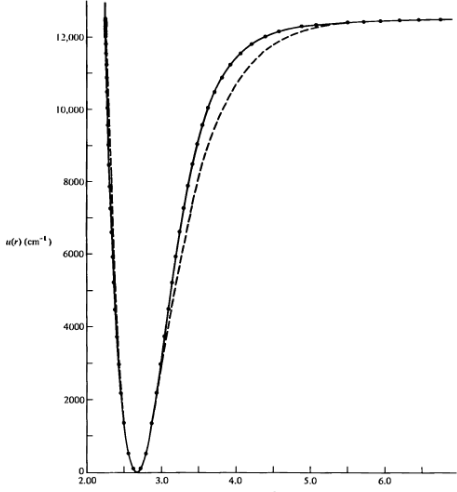
\includegraphics[width=0.6\linewidth]{interatomic_potential.png}
	\caption{Interatomic potential of a diatomic species.}
	\label{fig:diatomicpotential}
\end{figure}

\section{Rigid Rotor Harmonic Oscillator}%
\label{sec:RR}
For a diatomic atom, we first notice we can define translational movement as
that movement with respect to the center of mass, thus the Hamiltonian becomes
\begin{equation*}
	\mathcal{H} = \mathcal{H}_{trans} + \mathcal{H}_{int},
\end{equation*}
where the second term is the energy from the relative motion of the two masses.
This relative motion is clearly either rotational or vibrational. Technically
the rotational energy is effected by the current interatomic distance; however,
in most cases the changing of the effective radius is not consequential.

\textbf{Proof}
If we let $u(r)$ represent the interatomic potential, then a Taylor series
around the current distance, $R$, is,
\begin{align*}
	u(r) &= u(R) + (r - R)\left(\frac{\partial u}{\partial r}\right)_{r=R} +
	\frac{1}{2}(r - R)^2 \left(\frac{\partial^{2} u}{\partial
	r^2}\right)_{r=R}\\
		 &= u(R) + \frac{1}{2}k(r - R)^2.
\end{align*}
The second steps substitutes the second derivative for $k$. The reason we can
drop the linear term stems from the fact that in most cases the interatomic
distance is very close to the potential minimum. At the minimum, the first
derivative goes to zero. Therefore, if $k$ or the second derivative is large
then the bond is stiff and distance will not fluctuate much. \note%
that $k$ is similar to Hooke's constant.

We can then state,
\begin{equation*}
	\mathcal{H}_{int} = \mathcal{H}_{rot} + \mathcal{H}_{vib}.
\end{equation*}
Of course, the above is equivalent to,
\begin{equation*}
	q_{int} = q_{rot}q_{vib}.
\end{equation*}
This approximation is known as the rigid rotor harmonic oscillator
approximation. The approximation allows vibrational-rotational decoupling.

\section{Vibrational Partition Function}%
\label{sec:vib}
\subsection{Energy Levels and Spectra}
For a quantum harmonic oscillator, the energies are given by
\begin{equation*}
	\epsilon_{vib} = h\nu(n+ \frac{1}{2}).
\end{equation*}
\note that the degeneracy of each level is one, so each state is its
own level. $\nu$ is given by,
\begin{equation*}
	\nu = \frac{1}{2\pi} \left(\frac{k}{\mu}\right)^{1/2}.
\end{equation*}

The selection rules for vibrational transitions is that transitions can only
occur between energy adjacent states or $\Delta n = \pm 1$. Taking the above
equation for $\epsilon_{vib}$, and finding the energy difference between
adjacent levels gives
\begin{align*}
	\Delta\epsilon &= \epsilon_{n+1} - \epsilon_{n}\\
				   &= \nu h ((n + 3/2) - (n + 1/2)) = \nu h (1)\\
				   \nu\text{ then is,}\\
	\nu &= \frac{\Delta\epsilon}{h} =
	\frac{1}{2\pi}\left(\frac{k}{\mu}\right)^{1/2}.
\end{align*}
This gives the spectra for vibrational transitions. For there to be radiation, a
changing dipole in the molecule must exist. Using this equation, $k$ can be
found for different diatomic molecules. \textit{Note,} the vibrational spectra
consists of one line. One other quick fact is that for a given electronic state
there is an vibrational energy $D_o$ that corresponds to a disassociating
molecule. Figure~\ref{fig:diatomicelectronic} shows the potential the
vibrational mode operates in with some common quantities: $D_o$ represents the
dissociation energy for the molecule, $D_e$ represents the depth of the
potential well, the top function represents the first excited electronic state.
\begin{figure}[htpb]
	\centering
	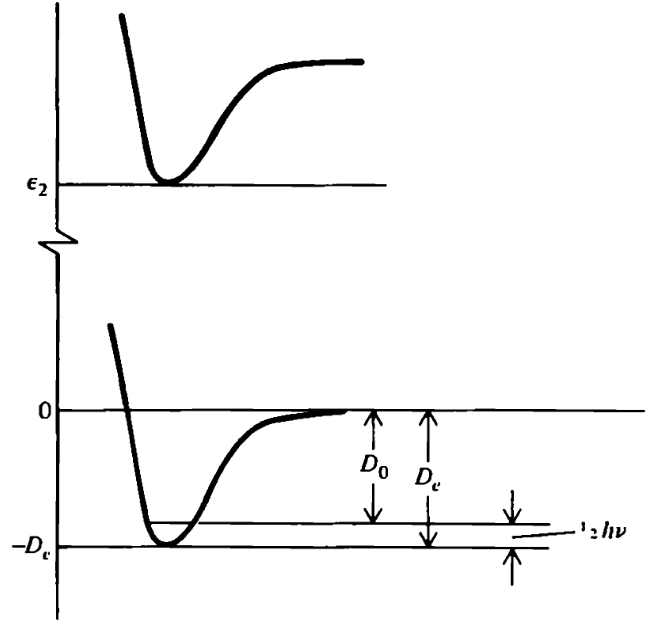
\includegraphics[width=0.7\linewidth]{electronic_states.png}
	\caption{Electronic potentials for the ground and first excited state with
	relevant quantities marked.}
	\label{fig:elecronic_states}
\end{figure}

\subsection{Deriving the Partition Function}
In order to derive the partition function, a zero state energy must be assigned.
Two possibilities exist 0 or $h\nu/2$. The book uses the latter and so shall I.
The derivation of the vibrational partition function goes as follows,
\begin{align*}
	q_{vib} &= \sum_{n}{e^{-\beta\epsilon_n}}\\
			&= \sum_{n}{e^{-\beta h\nu(n+1/2)}} = \sum_{n}{e^{-\beta h\nu
			n}e^{-\beta h\nu/2}}\\
			&= e^{-\beta h\nu/2}\sum_{n=0}^{\infty}{e^{-\beta h \nu n}}\\
			&= \frac{e^{-\beta h\nu/2}}{1 - e^{-\beta h \nu}} \qquad e^{-\beta h
			\nu} < 1.
\end{align*}
The first step follows by definition. The second is just the expansion and
simplification of $\epsilon_{vib}$. The third is just taking the constant out of
the sum. The fourth step involves seeing that the sum is a geometric series if
$e^{-\beta h \nu} < 1$. The partition function here is exact given the
constraint, but we can still take a high temperature limit using an integral.
This then is,
\begin{equation*}
	q_{vib} = e^{-\beta h\nu/2}\int_{n=0}^{\infty}{e^{-\beta h \nu n}\d n}
	= \frac{kT}{h\nu}.
\end{equation*}
\subsection{Properties of Vibrational Mode}
We will look at level occupancy and average vibrational energy. The average
energy given by the exact partition function is,
\begin{align*}
	E_v &= NkT^2 \frac{\d\ln q_v}{\d T} = NkT^2\frac{\d}{\d T}
	\left(\frac{h\nu}{2kT} - \ln{(1 - e^{-h\nu/kT})}\right)\\
		&= \frac{Nk\Theta}{2} + Nk\Theta \frac{e^{-\Theta/T}}{1 -
			e^{-\Theta/T}} = Nk\Theta \left(\frac{1}{2} + \frac{1}{e^{\Theta/T}
		-1}\right).
\end{align*}
Where, $\Theta = h\nu/k$. For the high temperature limit, we have,
\begin{equation*}
	E_v = NkT^2 \frac{\d\ln q_v}{\d T} = NkT^2 \frac{\d}{\d
	T}\left(\ln{\frac{T}{\Theta}}\right) = NkT.
\end{equation*}
The specific heat in this case is simply $Nk$ since $C_v$ is the derivative of
energy with respect to temperature.

The fraction of molecules in a given energy state are,
\begin{equation*}
	f_n = \frac{e^{-\beta h\nu (n+1/2)}}{q_{vib}}.
\end{equation*}
Therefore the fraction of molecules in an excited state are,
\begin{equation*}
	f_{n > 0} = \frac{\sum_{n=1}^{\infty}{e^{-\beta h\nu (n+1/2)}}}{q_{vib}} = 1
	- f_0 = \frac{e^{-\beta h\nu /2}}{q_{vib}} = 1 - (1 - e^{-\beta h \nu}) =
	e^{-\beta h \nu}.
\end{equation*}
The solution comes from the fact that the fraction in a excited state is the
inverse of the fraction in the ground state.

\section{Rotational Partition Function}%
\subsection{Energy States and Spectra}
\label{sec:rot}
For a rigid rotor the energy states and degeneracy are given by,
\begin{align*}
	\epsilon_j &= \frac{\hbar^2 J(J+1)}{2 I}\\
	\omega_j &= 2J+1.
\end{align*}
Here, $I$ is the moment of inertia, which is $\mu r_e^2 $ for the diatomic
case. $\mu$ is the reduced mass of the molecule. 

The transition rules for rotational energy are that the transition must be
adjacent like the vibrational modes and the molecule must have a permanent
dipole moment. The electromagnetic spectra that comes from the rotational energy
is then given by taking the different in adjacent energy levels like before.
\begin{align*}
	\Delta\epsilon &= \epsilon_{j+1} - \epsilon_j = \frac{\hbar^2}{2I} ((J+1)(J+2)
	- J(J+1)) = \frac{\hbar^2}{I} (J+1)\\
	\nu &= \frac{\Delta\epsilon}{h} = \frac{h}{4\pi^2 I}(J+1)
\end{align*}
To get the final form, $\hbar$ was expanded to $h/2\pi$. What this says is
unlike vibrational energy, rotational energy transitions emit multiple
wavelengths. \note we will set the rotational ground energy to zero.

\subsection{Deriving the Rotational Partition Function}
\subsection{Heteronuclear Derivation}
For reasons of wavefunction symmetry under the exchange of particles we must
separate the heteronuclear and homonuclear cases. We begin by examining the
heteronuclear.

By definition,
\begin{equation*}
	q_{rot} = \sum_{J=0}^{\infty}{(2J+1)e^{-\beta\bar{B}J(J+1)}}.
\end{equation*}
The variable $\bar{B}$ is $h/8\pi^2 Ic$ where c is the speed of light. Then,
$\epsilon_J = \bar{B}J(J+1)$. We can further define $\Theta_r$ to be $\bar{B}/k$
which is a rotational temperature. In order to write the summation in terms of a
integral we require that the difference between adjacent values be small. This
is fulfilled if $\Theta_r / k (J+1)$ is small which is true at small $J$. By the
time large $J$ are reached the contributions become negligible though, so we can
just take the integral.
\begin{align*}
	q_{rot} &= \int_0^{\infty}{(2J+1) e^{-\Theta_r J(J+1)/T} \d J}\\
			&= \int_0^{\infty}{e^{-\Theta_r J(J+1)/T} \d [J(J+1)]} = \left[
			\frac{T}{\Theta_r} e^{-\Theta_r J(J+1)/T}\right]_{0}^{\infty} =
			\frac{T}{\Theta_r}\\
			&= \frac{8\pi^2 IkT}{h^{2}}. 
\end{align*}
The second line recognizes that a change of variable can drastically simplify
the integral. For cases where the above is a bad approximation say $\Theta_r >
0.7T$, the summation can be expanded to 4 terms with good accuracy. Of course
higher order approximations can be taken.

The two approximation, however, leave an intermediate gap. The solution is to
use a Euler-MacLaurin summation formula approximation. This is given by
\begin{equation*}
	\sum_{n=a}^{b}{f(n)} = \int_{a}^{b}{f(n)\d n} + \frac{1}{2} [f(b)+f(a)] +
			\sum_{j=1}^{\infty}(-1)^{j}\frac{B_j}{(2j)!}[f^{(2j-1)}(a) -
			f^{(2j-1)}(b)],
\end{equation*}
where $B_j$ is the $j$-th Bernoulli number and the last bracketed term uses the
$(2j-1)$-th derivative. This give for the rotational partition function,
\begin{equation*}
	q_{rot} = \frac{T}{\Theta_r} \left( 1 +
		\frac{1}{3}\left(\frac{\Theta_r}{T}\right) +
		\frac{1}{15}\left(\frac{\Theta_r}{T}\right)^2 +
	\frac{1}{315}\left(\frac{\Theta_r}{T}\right)^3 + \cdots\right).
\end{equation*}

\subsection{Heteronuclear Thermodynamics}
The ensemble rotational energy in the high temperature limit is,
\begin{equation*}
	E_r = NkT^2 \left(\frac{\partial \ln q_{rot}}{\partial T}\right) = NkT^2
	\left(\frac{\partial}{\partial T}\right) (\ln T - \ln \Theta_r) = NkT.
\end{equation*}
This means that $C_v$ like in the vibrational case is $Nk$. The fraction of
molecules in a particular vibrational state can be taken just like the
rotational state, but since it is an identical procedure it is not shown here.
However, an important feature of rotational energy levels is that the most
occupied level at room temperature is an excited state. The most occupied level
can be derived by taking the derivative of the occupancy fraction,
\begin{equation*}
	\frac{\d f_J}{\d J} = \frac{\d}{\d J}\left(\frac{N_J}{N}\right) =
	\frac{\d}{\d J}\left(\frac{(2J+1)e^{-\Theta_r J(J+1)/T}}{q_{rot}}\right),
\end{equation*}
and setting it equal to zero.

\subsection{Homonuclear Derivation}
\note The homonuclear case can be approximated by
\begin{equation*}
	q_{rot,homo} = \frac{q_{rot,heter}}{2}.
\end{equation*}
This deals with the fact that in the homonuclear case a two-fold symmetry exists
perpendicular to the interatomic axis. This prevents the over counting of states.
This factor of 2 can be generalized to a factor $\sigma$ which is called the
symmetry number and represents the number of indistinguishable rotational states
or the number or rotational symmetries.

However, this will not work at low temperatures since homonuclear diatomic
molecules must obey certain wavefunction symmetries when an exchange of nuclei
is performed. This symmetry depends on the spins of the nuclei. If the spins are
integers the wavefunction is symmetric; otherwise, the wavefunction is
anti-symmetric with respect to exchange.

\subsubsection{Digression on Symmetry Requirements}
To determine the individual symmetry contributions of the electronic,
translational, vibrational, rotational, and nuclear energies to the
wavefunction, we imagine that we take a diatomic molecule and exchange both
nuclei along with their electrons. We then flip the electrons again. For
molecules where only the ground electronic state is useful and ground state is
$\Sigma_g^+$, the electronic wavefunction is symmetric to such operations. The
translational and vibration wavefunctions are obviously unaffected by such
transformations. This only leaves the nuclear and rotational.

By looking at the rotational wavefunctions for hydrogen, one can see that even
$J$ are symmetric to the swap, but odd $J$ are anti-symmetric to it. In
addition, for hydrogen, the nuclei spins are $\pm 1/2$. This leads to four spin
combinations: three are symmetric and one is anti-symmetric. Since the total
wavefunction must be anti-symmetric we must pair symmetric rotational
wavefunctions with anti-symmetric nuclear wavefunctions and vice versa. The
opposite holds true for integer spin molecules.

For a generic system the number of spin states for a nucleus is $2I+1$. For a
diatomic molecule there are $(2I+1)^2$ states then. The number of antisymmetric
states can be calculated using $(2I+1)(2I)/2$. The number of symmetric is just
the total minus the number of antisymmetric wavefunctions. This leads to
\begin{itemize}
	\item Integral spin
		\begin{itemize}
			\item Odd J - I(2I+1)
			\item Even J - (I+1)(2I+1)
		\end{itemize}
	\item Half-integral spin
		\begin{itemize}
			\item Odd J - (I+1)(2I+1)
			\item Even J - I(2I+1).
		\end{itemize}
\end{itemize}
One can see that the two are just mirrors of each other. The partition function
is then,
\begin{equation*}
	q_{rot,nucl} = w_{k,even}\sum_{J~even}{(2J+1)e^{-\Theta_r J(J+1)/T}} +
	w_{k,odd}\sum_{J~odd}{(2J+1)e^{-\Theta_r J(J+1)/T}},
\end{equation*}
where $w_{k,even/odd}$ represents the appropriate spin weighting. The rotation
and nuclear partition functions are then coupled. However, at high temperatures,
\begin{equation*}
	\sum_{J~odd} \approx \sum_{J~even} \approx \frac{1}{2}\sum_{J}.
\end{equation*}
This is just one half of the heteronuclear case. Then all the previous equations
apply with the adding factor of $1/2$. In this limit, we can separate the
partition functions to get,
\begin{align*}
	q_{rot} &= \frac{T}{2\Theta_r} = \frac{T}{\sigma\Theta_r}\\
	q_{nucl} &= (2I+1)^2.
\end{align*}
This requires that $\Theta_r < 0.2T$. $\sigma$ is just the symmetry number
mentioned previously. When the temperature is not high enough however the
coupled partition function must be used. In general, this is only necessary with
molecules like hydrogen where $\Theta_r$ is appreciable at gas temperatures. The
splitting of $H_2$ into two different types para (parallel spins) and ortho
(anti-parallel spins) comes from this weighting. At room temperature $H_2$ is
25\% para and 75\% ortho. At lower temperatures though this ratio changes as the
summations over even and odd $J$'s are not approximately equivalent.

All thermodynamic quantities can be calculated normally and will either not vary
in the high temperature limit (as is the case for energy and specific heat) or
will vary by factors of $\sigma$. This is also true in the Euler-MacLaurin
approximation.

\section{Total Partition Function}%
\label{sec:tpf}
The total partition function then becomes at the high temperature limit of the
harmonic-oscillator rigid rotor approximation,
\begin{align*}
	q &= q_{trans}~q_{rot}~q_{vib}~q_{nucl}~q_{elec}\\
	  &= \left(\frac{2\pi mkT}{h^2 }\right)^{3/2} V \frac{8\pi^2 IkT}{\sigma
	  h^{2}} \frac{e^{-\beta h\nu/2}}{1 - e^{-\beta h\nu}} \omega_{e1}
		  e^{D_e/kT}.
\end{align*}
This equation ignores the nuclear partition function.

\note In cases where the ground electronic state is not a $\Sigma$ state, the
electronic and nuclear angular momentum must be coupled. At high temperatures
compared to $\Theta_r$, they can still be decoupled, however. This means that
for all but low temperatures for molecules like NO the previous approach would
work.


\end{document}
